\providecommand{\main}{../../../..}
\documentclass[\main/dresen_thesis.tex]{subfiles}
\begin{document}
  \label{sec:colloidalCrystals:layers:xrr}
  \begin{figure}[tb]
    \centering
    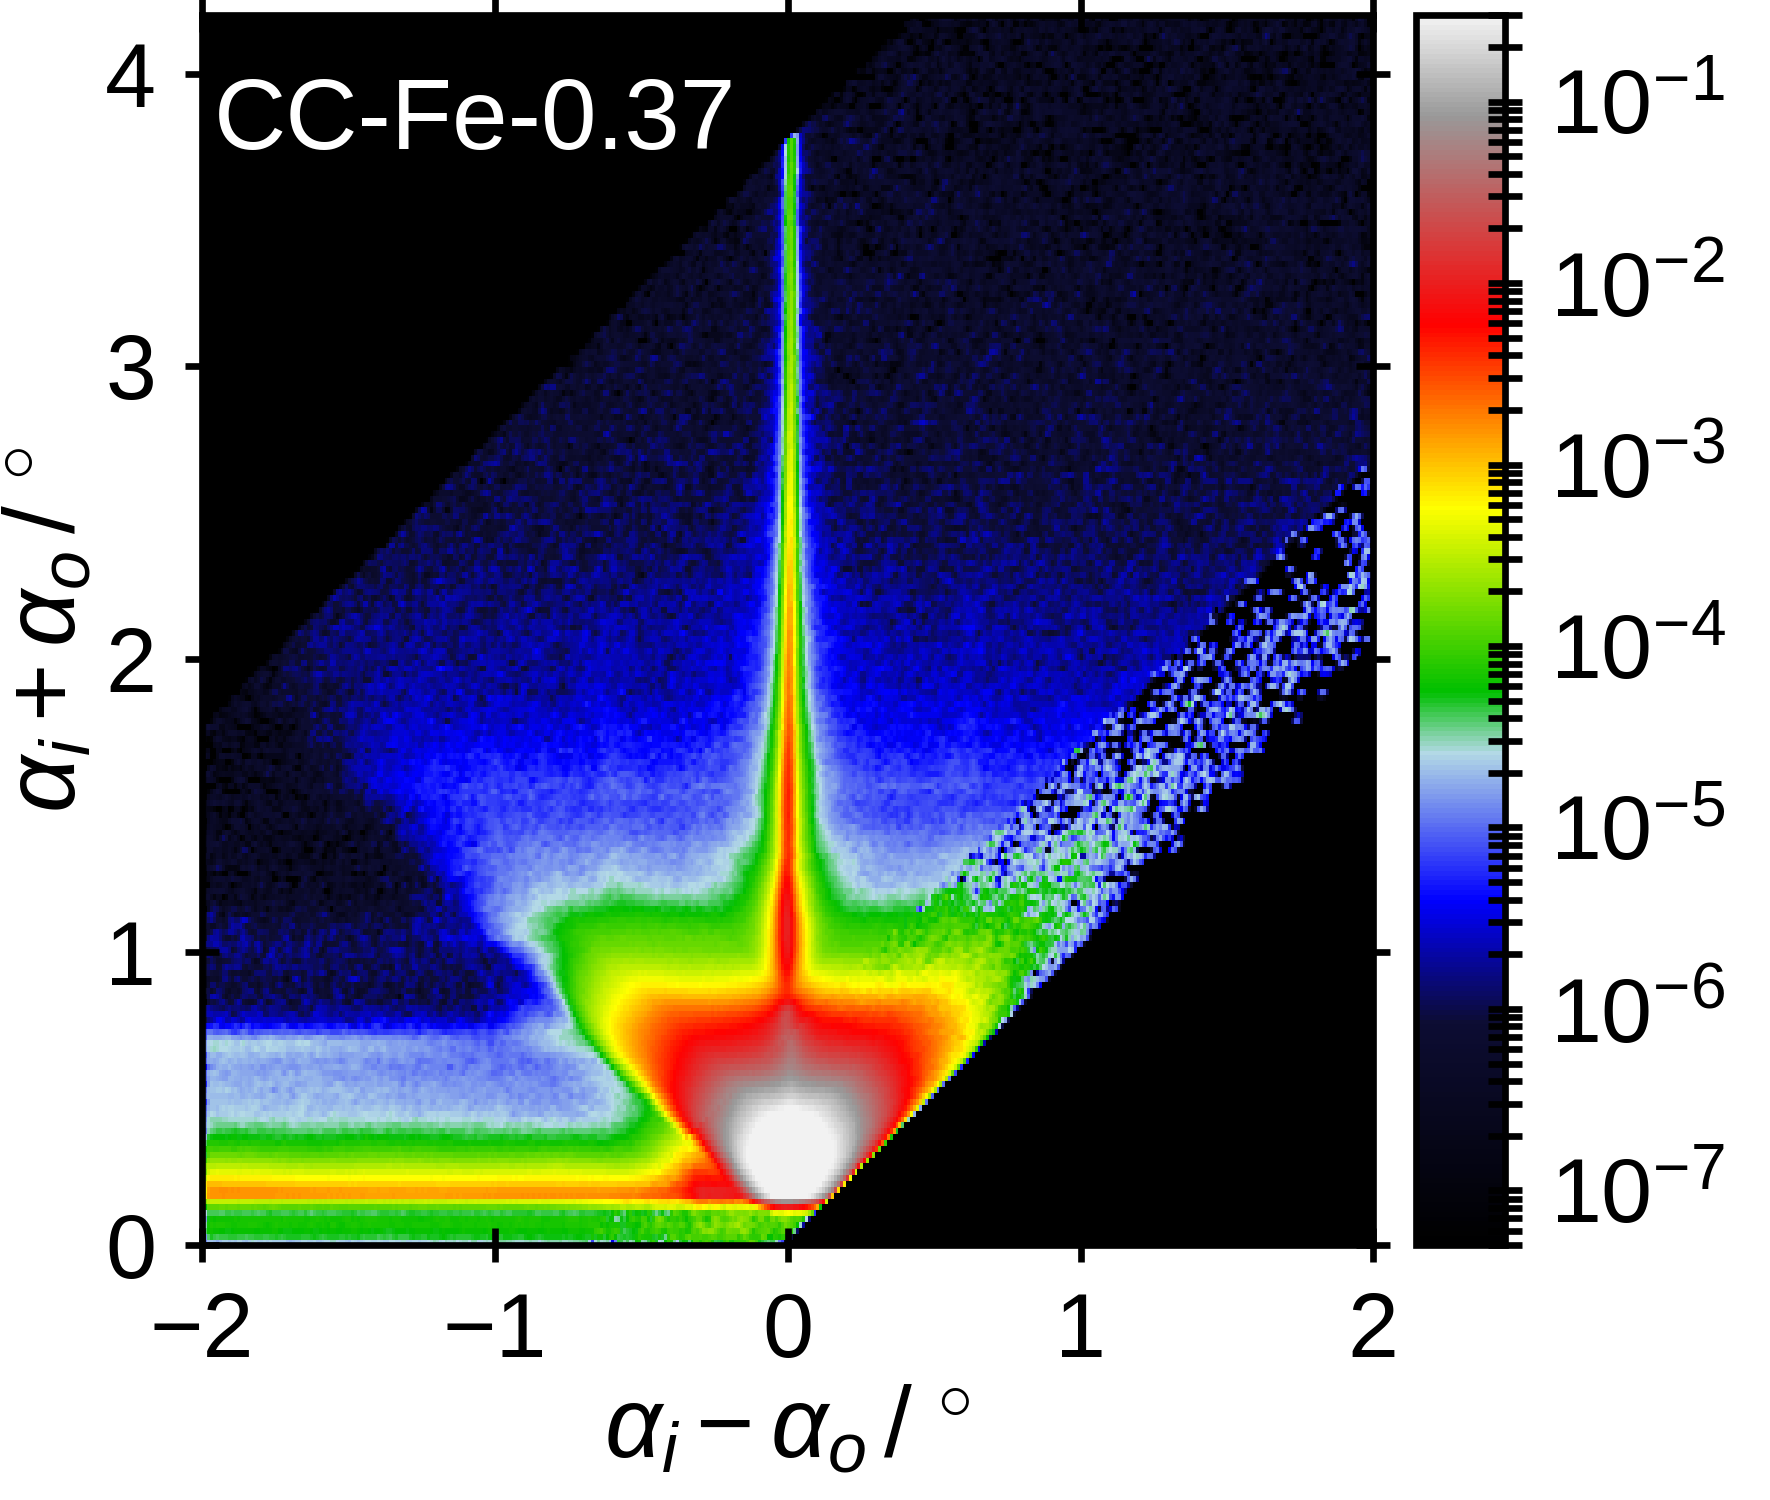
\includegraphics{colloidalCrystals_PNR_CC_Fe_0_37_ReflectivityMapXRR}
    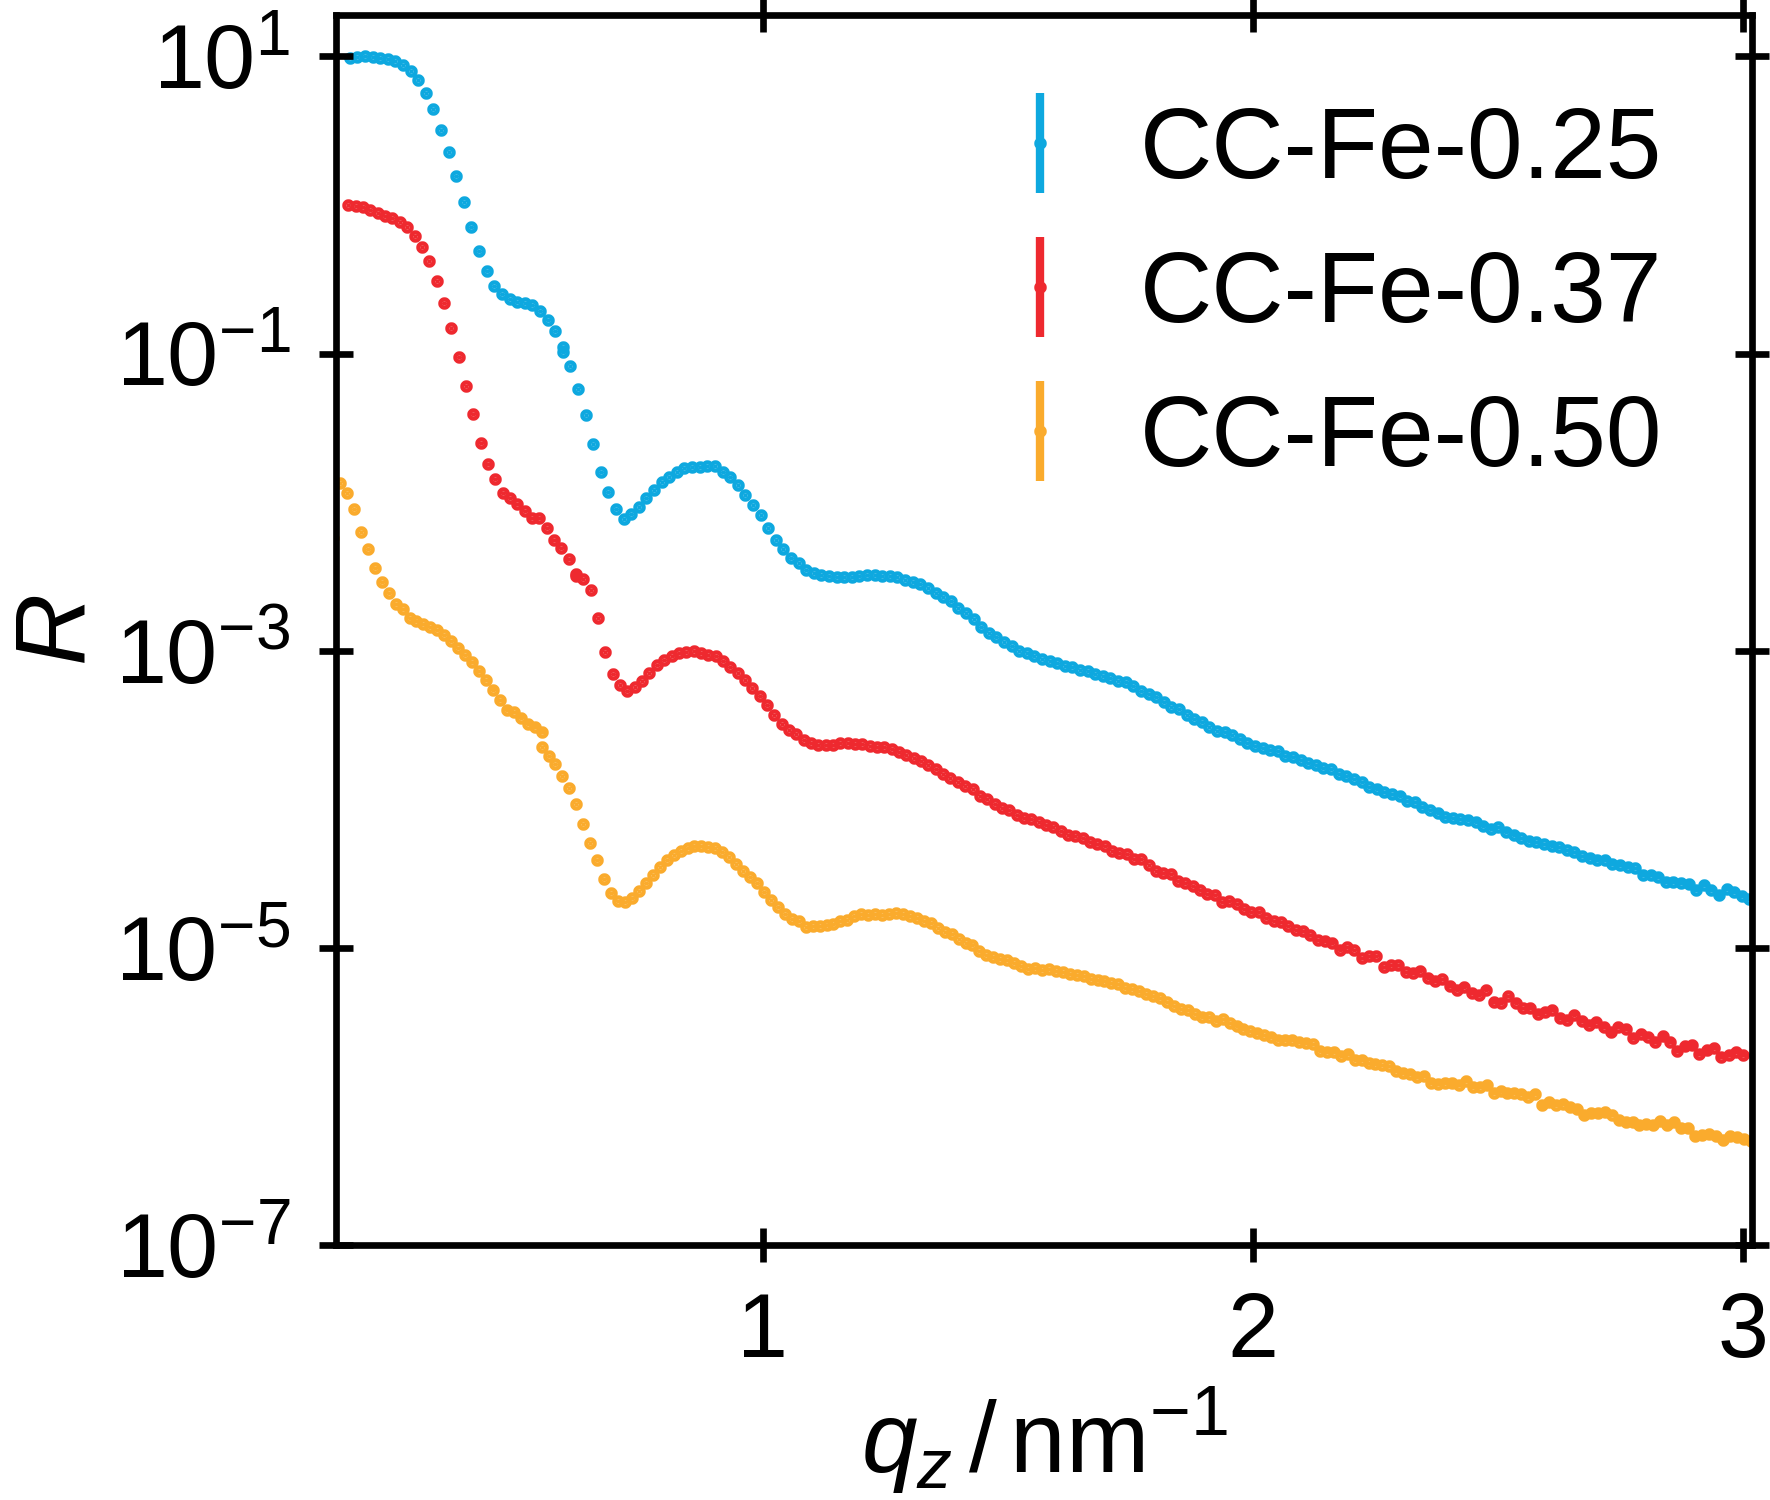
\includegraphics{colloidalCrystals_VerticalStructure_Combined_XRR}
    \caption{\label{fig:colloidalCrystals:xrr}X-ray reflectometry of CC-Fe-0.25, CC-Fe-0.37 and CC-Fe-0.50. Reducing the detector images, a reflectivity map is obtained, shown exemplary for CC-Fe-0.37 (left). Integrating a box around $\alpha_i - \alpha_o \eq 0 ^\circ$ and subtracting the diffuse scattering from the off-specular region, the specular reflectivity is obtained (right). The reflectivities of the samples are scaled by a factor of ten respectively for distinction.}
  \end{figure}

  The three samples CC-Fe-0.25, CC-Fe-0.37 and CC-Fe-0.50 have been studied by X-ray reflectometry using the GALAXI instrument.
  An exemplary reflectivity map for CC-Fe-0.37 and the reflectivities of all samples are shown for direct comparison in \reffig{fig:colloidalCrystals:xrr}.
  The reflectivity map shows the specular reflectivity line around $\alpha_i - \alpha_o \eq 0 ^\circ$ as region of strong intensity and additionally broad Bragg sheets in the off specular region.
  Slightly visible in the reflectivity map is also the overlap region of the two data sets, which were measured with varied counting time, which is an artifact from the edge region of the respective data sets and cleaned from the integrated reflectivity.

  Qualitatively, the three reflectivities show similar features with a correlation peak near $0.53 \unit{nm^{-1}}$, $0.87 \unit{nm^{-1}}$ and $1.23 \unit{nm^{-1}}$.
  From the period of the correlation peaks a length scale of $L \eq 18.0(5) \unit{nm}$ can be estimated.
  With increasing sample thickness, the plateau of total reflection is bends down in direct comparison from CC-Fe-0.37 to CC-Fe-0.25 and is not visible for the case of CC-Fe-0.50.
  Also with increasing sample thickness, the first peak around $0.53 \unit{nm^{-1}}$ smears out and becomes less well-defined.

  The reduced critical edge can be argumented by the larger thickness of iron oxide nanocube layers.
  The average scattering length density of the iron oxide layer can be lower than that of the silicon substrate ($\approx 20 \cdot 10^{-6} \angstrom^{-2}$, corresponding to $q_c \eq 0.3 \unit{nm^{-1}}$) and for an increasing thickness it becomes the determining density for the critical reflection condition.
  But even more important, iron oxide partially absorbs X-rays, which becomes apparent from the imaginary part of the scattering length density that is approximately $10 \%$ in magnitude of the real part.
  This leads to the observed rounding effect of the critical edge, where with increasing incident angle close to the critical edge the X-ray photons penetrate deeper into the layer and become partially absorbed.
  For the case of the complete vanishing of the critical edge for CC-Fe-0.50, it can however not completely excluded that an unknown mistake was performed during the alignment of the sample.

  Comparing the obtained vertical length scale from the correlation peaks to the nanocube size of $a \eq 12.26(4) \unit{nm}$ from SAXS in \refsec{sec:colloidalCrystals:nanoparticle:sas}, a ratio of $L/a \approx 1.47$ is observed, which is significantly larger than what could be expected from the edge length and additional interparticle spacing from the surfactant.
  Considering the face diagonal of the cubes $\sqrt{2} a \eq 17.33(6) \unit{nm}$, the length scale fits however closely, which connects to the observation from SEM in \refsec{sec:colloidalCrystals:layers:sem} that the cubes are rotated with their faces in respect to the substrate normal.

  Comparing the length scale to the $c\eq 51.3(5) \unit{nm}$ lattice constant observed in GISAXS, a ratio of  $c / L \approx 2.85$ is obtained.
  The length scale close to a ratio of $c/L \eq 3$ fits to the ($bct$) structure with [101] orientation as it is depicted in \reffig{fig:colloidalCrystals:layers:gisaxsBCTUCDepiction} and is therefore considered as supportive to the discussion in the GISAXS section.

  None of the reflectivities show defined Kiessig fringes, which could, however, still be expected from the observed sample thickness seen in SEM micrographs.
  Thus it can be concluded that a larger thickness variation is present in the sample, which would smear out the Kiessig fringes.
  This makes it additional complicated to determine the thickness from a qualitative discussion of the sample.
\end{document}